% !TEX root = ../dg.tex

\section{The Lie Bracket on Vector Fields}
\label{sec:Lie bracket of vector fields}

As we've defined it, $\mathfrak{X}(M)$ is a $C^\infty(M)$-module:\footnote{If you haven't seen modules before, they're basically like vector fields where the ring of scalars isn't necessarily a field. In the case of $\mathfrak{X}(M)$, the smooth functions $C^\infty(M)$ serve as the scalars, but $C^\infty(M)$ is only a ring, not a field: only nowhere-vanishing functions have well-defined inverses.}  we can certainly add two vector fields or multiply a vector field by a smooth function and get a new vector field.

In fact, there is even more algebraic structure on $\mathfrak{X}(M)$: it is something called a \emph{Lie algebra}, which means it is a (real) vector space which admits a binary operation (called a \emph{Lie bracket}) satisfying certain axioms.\footnote{Pronunciation note: The Norwegian surname ``Lie'' is typically pronounced the same as the common English or Korean surname ``Lee,'' rather than like the English word ``lie.''}

In order to define the Lie bracket of vector fields, it is instructive to think about how we could possibly define a binary operation on vector fields. For example, we could try to generalize binary operations on vector fields we already know in certain special cases. For example:
\begin{itemize}
	\item Since $T\R \cong \R \times \R$, we can interpret a vector field on $\R$ as a real-valued function by just recording the second entry: $X(p) = (p,v)$, and the corresponding function is $p \mapsto v$. Since functions form an algebra by pointwise multiplication, this defines a binary operation on vector fields on $\R$.
	
	\item More generally, every smooth 1-manifold has a trivial tangent bundle, so we can treat any vector field on any 1-manifold as a smooth, real-valued function and get an algebra structure on vector fields.\footnote{This correpondence between sections of trivial line bundles and functions gives you some reason to believe that the appropriate notion of ``function'' in algebraic geometry is often a section of a line bundle.}
	
	\item Since $T \R^2 \cong \R^2 \times \R^2$ and since we can define an equivalence $\R^2 \leftrightarrow \C$ by $(x,y) \leftrightarrow x + iy$, we can interpret a vector field on $\R^2$ (or, more generally, any surface with trivial tangent bundle) as a complex-valued function. Again, functions form an algebra by pointwise multiplication, so this defines a binary operation on vector fields on $\R^2$.\footnote{Interpreting vector fields on the plane as complex-valued functions turns out to be quite useful in 2-dimensional fluid mechanics; look up \emph{stream function} and \emph{complex potential} for more.}
	
	\item Since $T\R^3 \cong \R^3 \times \R^3$, we can interpret a vector field on $\R^3$ as a vector-valued function on $\R^3$. Then the (pointwise) cross product $\times$ gives a binary operation on vector fields on $\R^3$.
	
	\item Since $T\R^4 \cong \R^4 \times \R^4$ and since we can define an equivalence $\R^4 \leftrightarrow \mathbb{H}$ between $\R^4$ and the quaternions by $(t,x,y,z) \leftrightarrow t +i x + j y + kz$, we can interpret vector fields on $\R^4$ as quaternion-valued functions. Again, functions form an algebra by pointwise multiplication, so this defines a binary operation on vector fields on $\R^4$. 
	
	This is in some sense a generalization of the cross product on $\R^3$: if we represent $(x,y,z),(u,v,w) \in \R^3$ by purely imaginary quaternions $p = ix + jy + kz$ and $q = iu + jv + kw$, then the quaternion product
	\[
		pq = -p \cdot q + p \times q,
	\]
	where $p \cdot q$ is the dot product of the two vectors in $\R^3$, and $p \times q$ is the cross product (interpreted as a purerly imaginary quaternion).\footnote{Look up \emph{Clifford algebras} for a vast generalization of this kind of product operation that splits into a scalar part (the $-p \cdot q$) and a vector part (the $p \times q$).}
\end{itemize}

So the natural question is: can we generalize these examples to higher-dimensional Euclidean spaces, and more generally to arbitrary manifolds?

Unfortunately, the answer is basically ``no.'' As you might have heard, there are no normed division rings over $\R$ besides $\R$, $\C$, and $\mathbb{H}$, and there aren't even normed division algebras (where we allow multiplication to be non-associative) aside from these examples and the octonions $\mathbb{O}$, which are 8-dimensional. 

Moreover, even if there were more normed division algebras, the operations above depended very strongly on the triviality of the tangent bundle, which is not going to work in more general manifolds.

So here's a different approach: recall that we can interpret vector fields on $M$ as operators on $C^\infty(M)$. That is, for $f \in C^\infty(M)$, $Xf \in C^\infty(M)$ as well; this is basically the function recording the directional derivative of $f$ in the direction of $X$ at each point on the manifold.

An obvious thing to guess is that, if $X,Y \in \mathfrak{X}(M)$, then the composition $X \circ Y = XY$ is also a vector field. After all, $(XY)f = X(Yf)$ \emph{will} be a smooth function, so $XY$ is also an operator on $C^\infty(M)$.

Let's work in local coordinates at a point $p \in M$ to see what this operator looks like when applied to a function $f$ which is differentiable at $p$.

We know that, in terms of the local coordinate basis $\left\{ \frac{\partial}{\partial x_1},\dots , \frac{\partial}{\partial x_n}\right\}$, we can write
\[
	X(p) = \sum_{i=1}^n a_i(p) \frac{\partial}{\partial x_i} \quad \text{and} \quad Y(p) = \sum_{i=1}^n b_i(p) \frac{\partial}{\partial x_i},
\]
where the $a_i$ and $b_i$ are smooth functions defined in some neighborhood of $p$. So then
\[
	(XY)f = X(Yf) = X\left(\sum_{i=1}^n b_i \frac{\partial f}{\partial x_i}\right) = \sum_{i,j=1}^n a_j \frac{\partial}{\partial x_j} \left( b_i \frac{\partial f}{\partial x_i}\right) = \sum_{i,j=1}^n a_j \left( \frac{\partial b_i}{\partial x_j}\frac{\partial f}{\partial x_i} + b_i \frac{\partial^2 f}{\partial x_j \partial x_i}\right).
\]

This should give you pause because it is no longer a first-order differential operator. Let's make this more obvious by rewriting as
\begin{equation}\label{eq:product of vector fields}
	(XY)f = \left[ \sum_{j=1}^n \left(a_j \left( \sum_{i=1}^n \frac{\partial b_i}{\partial x_j} \frac{\partial}{\partial x_i}\right)\right) + \sum_{j=1}^n \left(a_j \left(\sum_{i=1}^n b_i \frac{\partial^2}{\partial x_j \partial x_i}\right)\right)\right]f,
\end{equation}
so the stuff inside the brackets (which is $XY$) is a differential operator on $C^\infty(M)$, but it's not a vector field; for example, it cannot be written in terms of the local coordinate basis $\left\{ \frac{\partial}{\partial x_1}, \dots , \frac{\partial}{\partial x_n}\right\}$.

\begin{example}
	If $X = \frac{\partial}{\partial x}$ and $Y = \frac{\partial}{\partial y}$ are the standard coordinate vector fields on $\R^2$, then \eqref{eq:product of vector fields} reduces to
	\[
		(XY)f = \frac{\partial^2 f}{\partial x \partial y},
	\]
	as you would expect from computing
	\[
		X(Yf) = \frac{\partial}{\partial x} \left( \frac{\partial f}{\partial y}\right) = \frac{\partial^2 f}{\partial x \partial y}.
	\]
	So $XY = \frac{\partial^2}{\partial x \partial y}$. But there's no sensible way to interpret this second-order operator as a vector field.
\end{example}

\begin{example}\label{ex:radial and rotational fields}
	If $X = r \frac{\partial}{\partial r}$ and $Y = r \frac{\partial}{\partial \theta}$ are the (scaled) radial and rotational fields, then
	\[
		(XY)f = X(Yf) = r \frac{\partial }{\partial r} \left( r \frac{\partial}{\partial \theta}f \right) = r \frac{\partial f}{\partial \theta} + r^2 \frac{\partial f}{\partial r \partial \theta},
	\]
	so
	\[
		XY = r \frac{\partial}{\partial \theta} + r^2 \frac{\partial}{\partial r \partial \theta}.
	\]
	Again, a second-order operator appears.
\end{example}

The problem with \eqref{eq:product of vector fields} is the second term, which is a second-order operator. Now notice that if we had done this in the reverse order we would have gotten
\begin{equation}\label{eq:product of vector fields 2}
	(YX)f = \left[ \sum_{j=1}^n \left(b_j \left( \sum_{i=1}^n \frac{\partial a_i}{\partial x_j} \frac{\partial}{\partial x_i}\right)\right) + \sum_{j=1}^n \left(b_j \left(\sum_{i=1}^n a_i \frac{\partial^2}{\partial x_j \partial x_i}\right)\right)\right]f.
\end{equation}
This doesn't just have the same type of problem as before, it has literally the same problem: because mixed partials commute, the second terms in \eqref{eq:product of vector fields} and \eqref{eq:product of vector fields 2} agree. So, by subtracting, we can cancel them and get
\begin{equation}\label{eq:Lie bracket in local coords}
	(XY - YX)f = \left[\sum_{i,j=1}^n \left(\left( a_j \frac{\partial b_i}{\partial x_j} - b_j \frac{\partial a_i}{\partial x_j}\right)\frac{\partial}{\partial x_i}\right)\right]f,
\end{equation}
which \emph{is} written in terms of the $\left\{ \frac{\partial}{\partial x_1}, \dots , \frac{\partial}{\partial x_n}\right\}$ basis. So this really \emph{is} a vector field.

\begin{definition}\label{def:Lie bracket of vector fields}
	If $X,Y \in \mathfrak{X}(M)$, the \emph{Lie bracket} of $X$ and $Y$ is a vector field $[X,Y]$ defined by
	\[
		[X,Y]f := X(Yf)-Y(Xf).
	\]
\end{definition}

The key feature of this operation is that it satisfies the axioms of a Lie bracket (\ref{it:Lie bracket anticommutativity}--\ref{it:Lie bracket Jacobi identity} in \Cref{prop:Lie bracket}), and hence makes $\mathfrak{X}(M)$ into a \emph{Lie algebra}.

\begin{proposition}\label{prop:Lie bracket}
	If $X,Y,Z \in \mathfrak{X}(M)$ and $a,b \in \R$, $f, g \in C^\infty(M)$, then
	\begin{enumerate}
		\item \label{it:Lie bracket anticommutativity} $[X,Y]=-[Y,X]$ (anti-commutativity)
		\item \label{it:Lie bracket linearity} $[aX+bY,Z]=a[X,Z]+b[Y,Z]$ (linearity)
		\item \label{it:Lie bracket Jacobi identity} $[[X,Y],Z]+[[Y,Z],X]+[[Z,X],Y]=0$ (Jacobi identity)
		\item $[fX,gY]=fg[X,Y]+f(Xg)Y-g(Yf)X$.
	\end{enumerate}
\end{proposition}

\begin{proof}
	Homework.
\end{proof}

\begin{example}
	Continuing with \Cref{ex:radial and rotational fields}, we already computed $XY$, so we can also compute 
	\[
		YX = r \frac{\partial}{\partial \theta} \left( r \frac{\partial}{\partial r}\right) = r^2 \frac{\partial^2}{\partial \theta \partial r},
	\]
	and hence
	\[
		[X,Y] = r \frac{\partial}{\partial \theta}.
	\]
\end{example}

\begin{example}
	Consider $M = S^2$ and the vector fields $X = \frac{\partial}{\partial \theta}$ and $Y = \frac{\partial}{\partial z}$ where $(\theta,z)$ are cylindrical coordinates on $S^2$; see \Cref{fig:dtheta and dz}. 
	
	\begin{figure}[htbp]
		\centering
			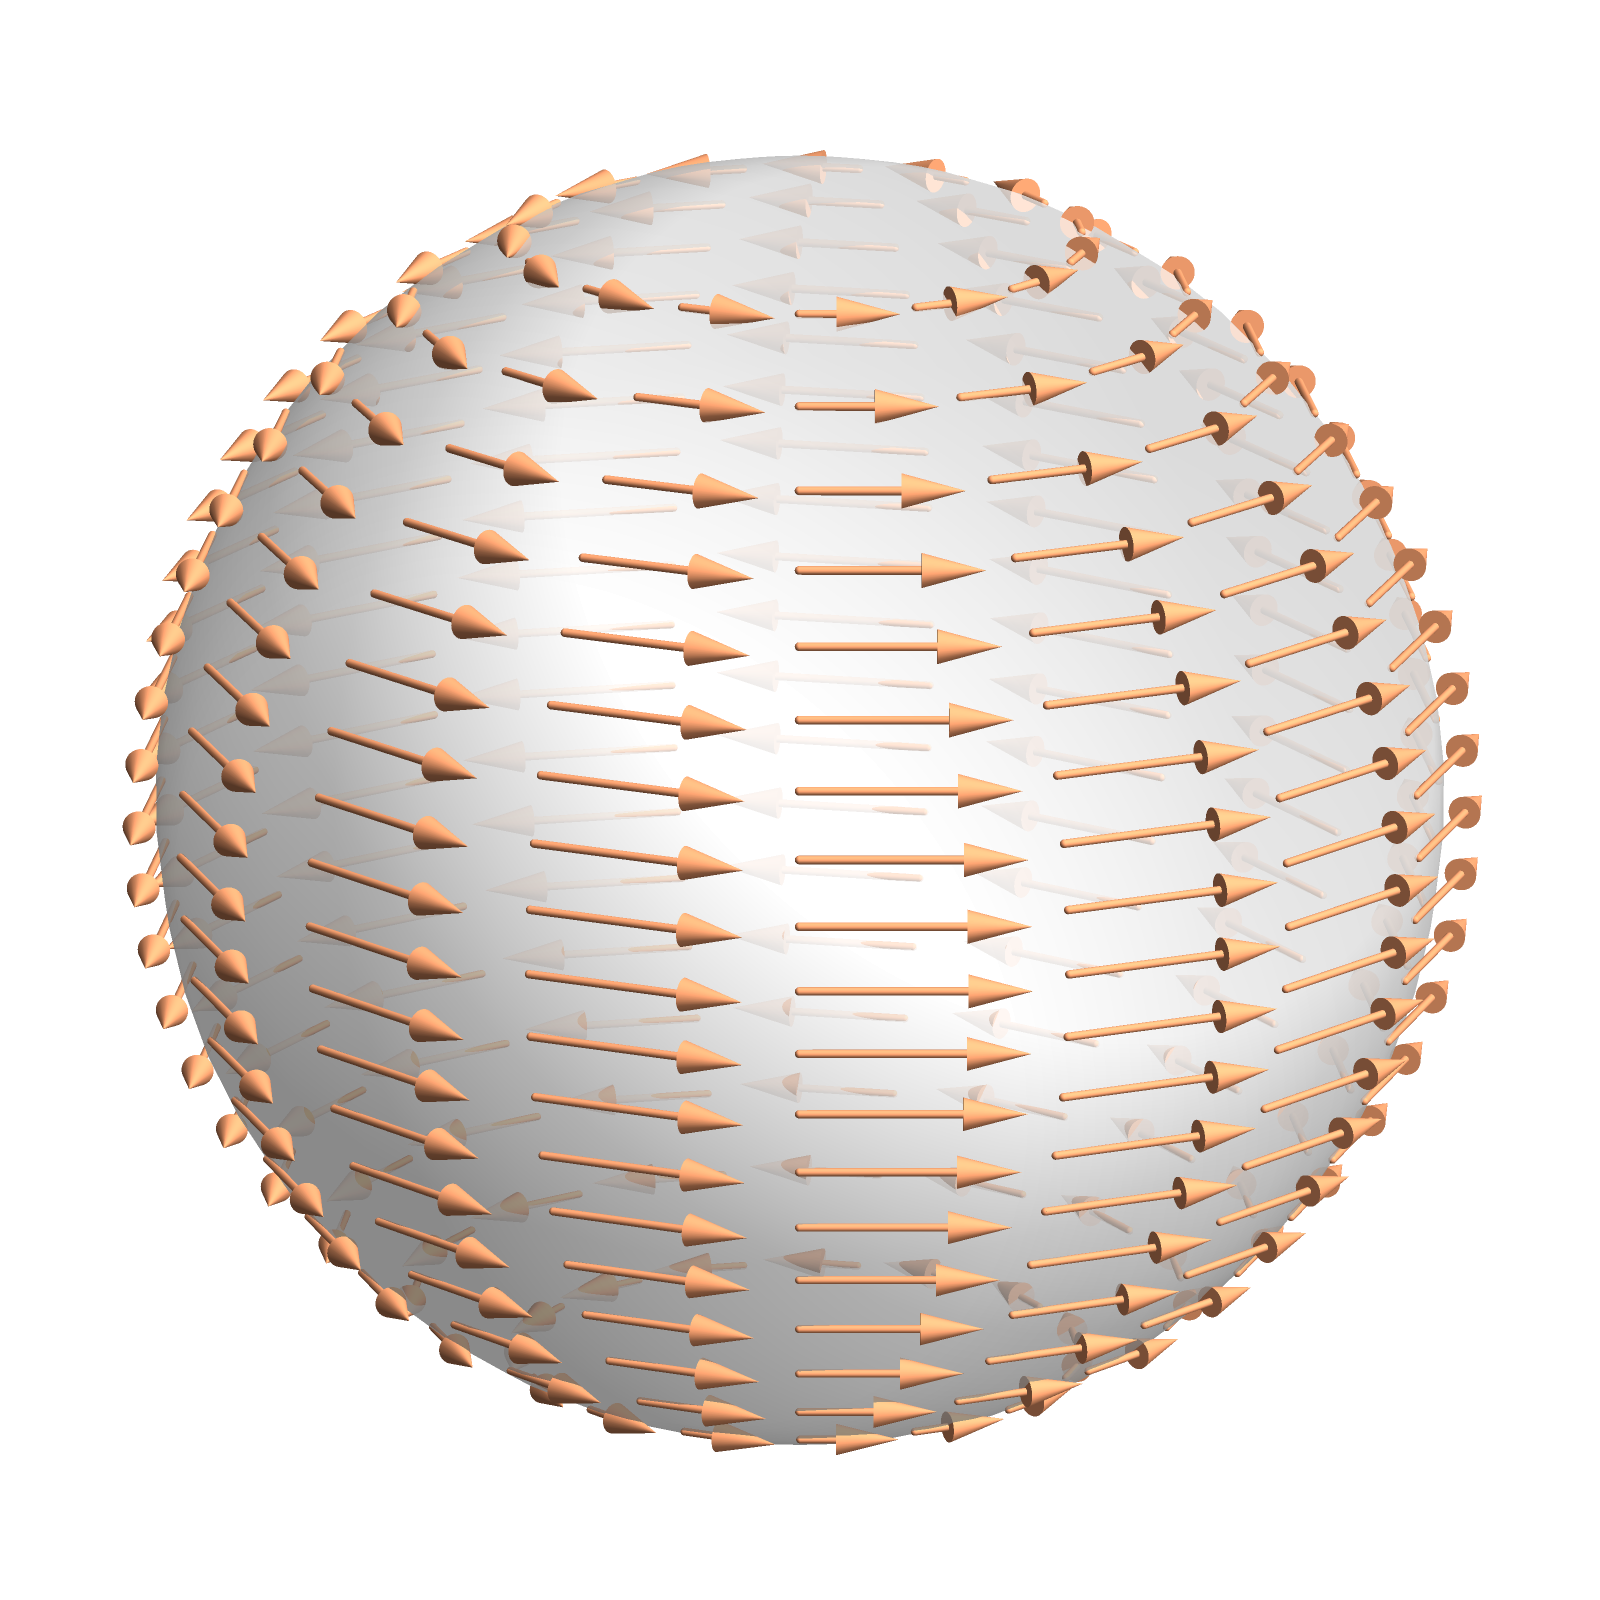
\includegraphics[height=2in]{dtheta} \qquad 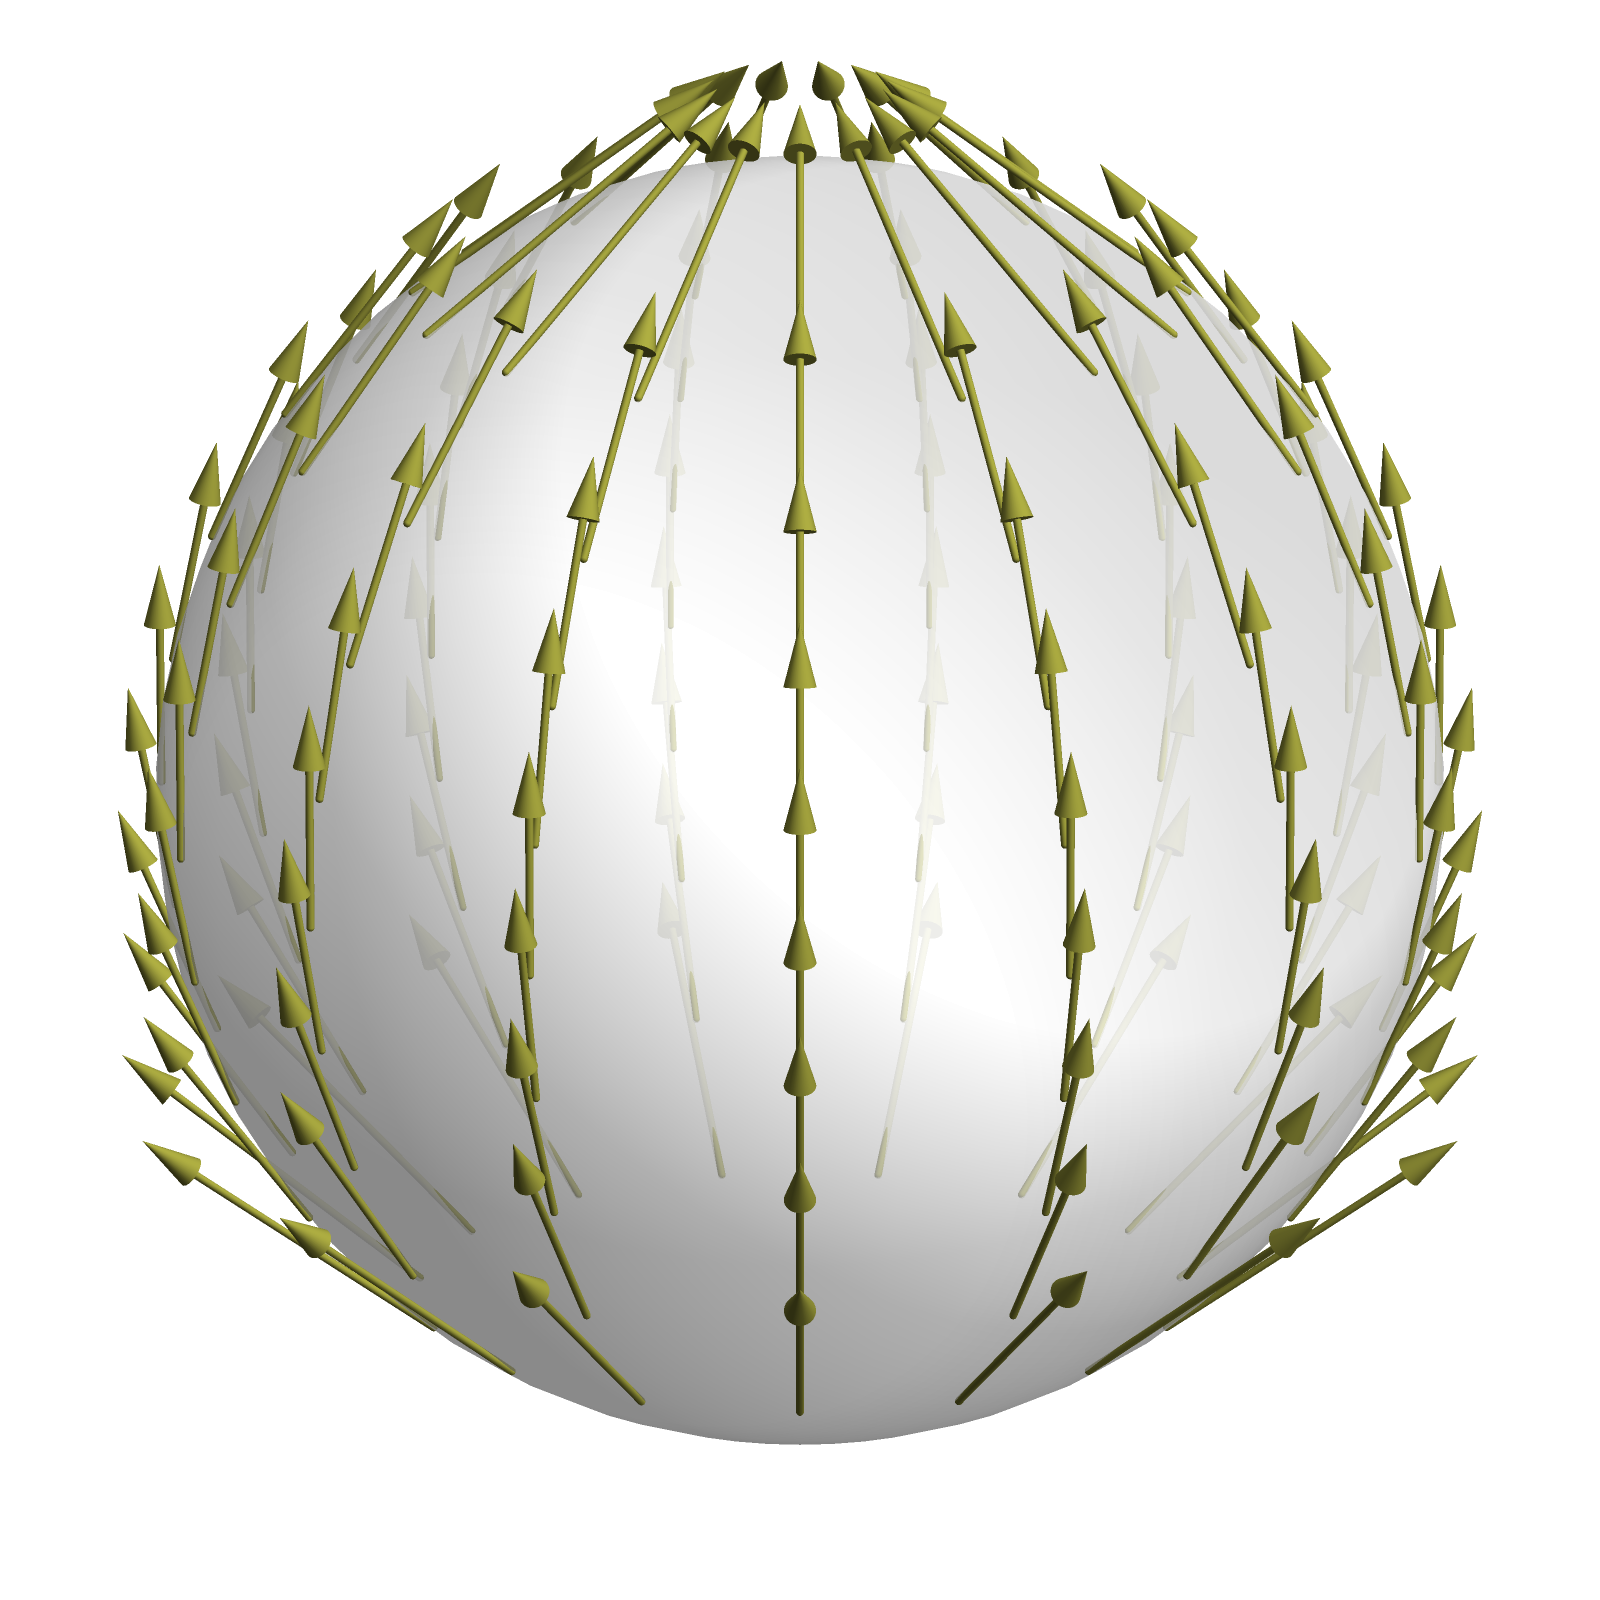
\includegraphics[height=2in]{dz}
		\caption{The vector fields $X = \frac{\partial}{\partial \theta}$ and $Y = \frac{\partial}{\partial z}$ on $S^2$.}
		\alttext{Two computer-generated semi-transparent gray spheres. On the left, a collection of orange arrows or shown on the sphere: the arrows point along circles of latitude: the lengths get shorter as they move away from the equator. On the right, there is a collection of green arrows on the sphere which point towards the north pole. The green arrows get longer as they get further from the equator.}
		\label{fig:dtheta and dz}
	\end{figure}
	
	In other words, we have the local coordinate chart $\phi\from (0,2\pi) \times (-1,1) \to S^2$ given by
	\[
		\phi(\theta,z) = (\sqrt{1-z^2} \cos\theta, \sqrt{1-z^2} \sin \theta, z),
	\]
	and $X$ and $Y$ are the corresponding coordinate fields.
	
	Notice that
	\[
		[X,Y]f = \frac{\partial^2 f}{\partial \theta \partial z} - \frac{\partial^2 f}{\partial z \partial \theta} = 0
	\]
	since mixed partials commute.
	
	More generally, whenever $X = \frac{\partial}{\partial x_i}$ and $Y = \frac{\partial}{\partial x_j}$ are coordinate fields in a neighborhood of a point in a manifold, $[X,Y] = 0$.
	
	In Cartesian coordinates
	\[
		X = \sqrt{1-z^2}\left( - \sin \theta \frac{\partial}{\partial x} + \cos \theta \frac{\partial}{\partial y}\right) = \sqrt{1-z^2}\left( - y \frac{\partial}{\partial x} + x \frac{\partial}{\partial y}\right),
	\]
	and
	\[
		Y = -\frac{z \cos\theta}{\sqrt{1-z^2}}\frac{\partial}{\partial x} - \frac{z \sin\theta}{\sqrt{1-z^2}}\frac{\partial}{\partial y} + \frac{\partial}{\partial z} = -\frac{xz}{1-z^2}\frac{\partial}{\partial x} - \frac{yz}{1-z^2}\frac{\partial}{\partial y} + \frac{\partial}{\partial z}.
	\]
	
	So then some much more unpleasant calculations using \eqref{eq:Lie bracket in local coords} shows you that $[X,Y] = 0$ in these coordinates as well.
\end{example}

Now we look at some examples of Lie algebras not coming from vector fields.

\begin{example}\label{ex:R^3 Lie algebra}
	$\R^3$ forms a Lie algebra with the bracket operation given by the cross product: for $u,v \in \R^3$, define $[u,v] := u \times v$. Then it is straightforward to check that this bracket satisfies \ref{it:Lie bracket anticommutativity}--\ref{it:Lie bracket Jacobi identity} above. Written in terms of cross products, \ref{it:Lie bracket Jacobi identity} says
	\[
		0 = (u \times v) \times w + (v \times w) \times u + (w \times u) \times v = (u \times v) \times w - u \times (v \times w) + v \times (u \times w),
	\]
	or equivalently,
	\[
		(u \times v) \times w = u \times (v \times w) - v \times (u \times w).
	\]
	In particular, this records the failure of associativity of the cross product.
\end{example}

More generally, the Jacobi identity records the failure of associativity of the Lie bracket:
\[
	[[X,Y],Z] = [X,[Y,Z]] - [Y,[X,Z]].
\]

\begin{example}\label{ex:Lie algebra U(d)}
	Recall \Cref{ex:left invariant vector field}, in which we showed that left-invariant vector fields on $\U(d)$ are of the form $X(U) = U \Delta_X$, for $\Delta_X \in T_I\U(d)$, which is the collection of skew-Hermitian $d \times d$ matrices. In particular, $X(I) = \Delta_X$.
	
	As we will see in more detail later (\Cref{prop:matrix group commutator}), it will turn out that the Lie bracket on left-invariant vector fields on a matrix group like $\U(d)$ just corresponds to the matrix commutator operation in the tangent space to the identity. 
	
	In this case, that means that, if $X,Y \in \mathfrak{X}(U(d))$ are left-invariant, then $[X,Y]$ is also left-invariant and, for each $U \in \U(d)$,
	\[
		[X,Y](U) = U(\Delta_X \Delta_Y - \Delta_Y \Delta_X),
	\]
	where the products inside parentheses are just matrix products between the skew-Hermitian matrices $\Delta_X$ and $\Delta_Y$; that is, the term in parentheses is just the usual matrix commutator.
	
	\begin{exercise}
		Check that the commutator of two skew-Hermitian matrices is skew-Hermitian.
	\end{exercise}
	
	This all tells you that the correspondence between left-invariant vector fields and elements of $T_I\U(d)$ turns the Lie bracket of left-invariant vector fields into the matrix commutator in $T_I \U(d)$. These are two different realizations of the same Lie algebra, usually called $\mathfrak{u}(d)$.
\end{example}

\begin{example}\label{ex:so3 Lie algebra}
	If we play the same game with $\SO(d)$, it turns out that the tangent space to the identity consists of $d \times d$ skew-symmetric matrices, and the Lie algebra on left-invariant vector fields on $\SO(d)$ corresponds to the matrix commutator on skew-symmetric matrices; we'll write the collection of skew-symmetric $d \times d$ matrices as $\mathfrak{so}(d)$.
	
	Consider the case $d = 3$. Then we can write elements of $\mathfrak{so}(3)$ as 
	\[
		\Delta = \begin{bmatrix} 0 & -z & y \\ z & 0 & -x \\ -y & x & 0 \end{bmatrix}.
	\]
	(The reason for the funny ordering and sign choices will shortly become apparent.)
	
	Now, $\mathfrak{so}(3)$ is a 3-dimensional vector space, and we have a vector space isomorphism $F\from \R^3 \to \mathfrak{so}(3)$ given by
	\begin{equation}\label{eq:r3 so3 isomorphism}
		F \from (x,y,z) \mapsto \begin{bmatrix} 0 & -z & y \\ z & 0 & -x \\ -y & x & 0 \end{bmatrix}.
	\end{equation}
	
	Let $\Delta_1,\Delta_2 \in \mathfrak{so}(3)$ with 
	\[
		\Delta_i = \begin{bmatrix} 0 & -z_i & y_i \\ z_i & 0 & -x_i \\ -y_i & x_i & 0 \end{bmatrix}.
	\]
	Then
	\[
		[\Delta_1, \Delta_2] = \Delta_1 \Delta_2 - \Delta_2 \Delta_1 = \begin{bmatrix} 0 & x_2 y_1-x_1 y_2 & x_2 z_1-x_1 z_2 \\
 x_1 y_2-x_2 y_1 & 0 & y_2 z_1-y_1 z_2 \\
 x_1 z_2-x_2 z_1 & y_1 z_2-y_2 z_1 & 0 \end{bmatrix}.
	\]
	
	If you stare at this, you might recognize the entries as being the coordinates of the cross product of the corresponding vectors:
	\[
		\begin{bmatrix} x_1 \\ y_1 \\ z_1 \end{bmatrix} \times \begin{bmatrix} x_2 \\ y_2 \\ z_2 \end{bmatrix} = \begin{bmatrix} y_1 z_2-y_2 z_1 \\ x_2 z_1-x_1 z_2 \\ x_1 y_2-x_2 y_1 \end{bmatrix}.
	\]
	In other words, $F(v_1 \times v_2) = [F(v_1), F(v_2)]$, so $F$ is a Lie algebra homomorphism. Since it's also a bijective linear map, it's a Lie algebra isomorphism, so we've just proved that $(\R^3, \times) \cong \mathfrak{so}(3)$ as Lie algebras.
	
	Thus, the Lie bracket on vector fields on manifolds is some sort of vast generalization of the cross product on $\R^3$. In this interpretation, $\R^3 \cong \mathfrak{so}(3)$ is the collection of infinitesimal rotations of 3-space, where $v \in \R^3$ corresponds to an infinitesimal rotation around the axis spanned by $v$, and the correspondence between cross products and commutators reflects the fact that, for very small $\epsilon > 0$ and unit vectors $u$ and $v$, the composition of an $\epsilon$-rotation around $u$ with an $\epsilon$-rotation around $v$ is, to first order, a rotation around $u + v + \frac{\epsilon}{2} u \times v$; see the Baker--Campbell--Hausdorff formula~\cite[Chapter~5]{hallLieGroupsLie2015}.
\end{example}

\begin{exercise}
	Convince yourself that, for $v \in \R^3$ a unit vector and $F$ as defined in \eqref{eq:r3 so3 isomorphism}, $\exp (F(\theta v))$ gives the one-parameter subgroup of rotations by angle $\theta$ around the axis spanned by $v$. (A full proof is kind of annoying to write down, but at least convince yourself this is true when $v$ is a coordinate vector.)
\end{exercise}